% \documentclass[dvipdfmx]{beamer}
\documentclass{beamer}
\usetheme{Antibes}

\usepackage{amssymb, amsmath, mathrsfs}
\usepackage{amsthm}
\usepackage{graphicx}
\usepackage{color}
\usepackage{subfigure}
\usepackage{animate}

\theoremstyle{remark}
\newtheorem{remark}[theorem]{Remark}

\newcommand{\abs}[1]{\lvert#1\rvert}
\newcommand{\norm}[1]{\lVert#1\rVert}
\DeclareMathOperator{\re}{Re}
\DeclareMathOperator{\im}{Im}
\newcommand{\ud}{\mathrm{d}}
\newcommand{\e}{\mathrm{e}}
\renewcommand{\i}{\mathrm{i}}

\begin{document}

\begin{frame}
	
	\title{Comparison of Continuum and Atomistic Models for Chemical Diffusion and Phase Separation}
	\date{\today}
	\author{Isaac Viviano}

	\maketitle

\end{frame}

\begin{frame}
	
	\tableofcontents

\end{frame}

\section{Chemical}

\begin{frame}{Diffusion}

	\begin{itemize}
		\item 
	\end{itemize}
	
\end{frame}

\begin{frame}{Phase Separation}
	
	quantified by order parameter
	
	\begin{figure}
		% 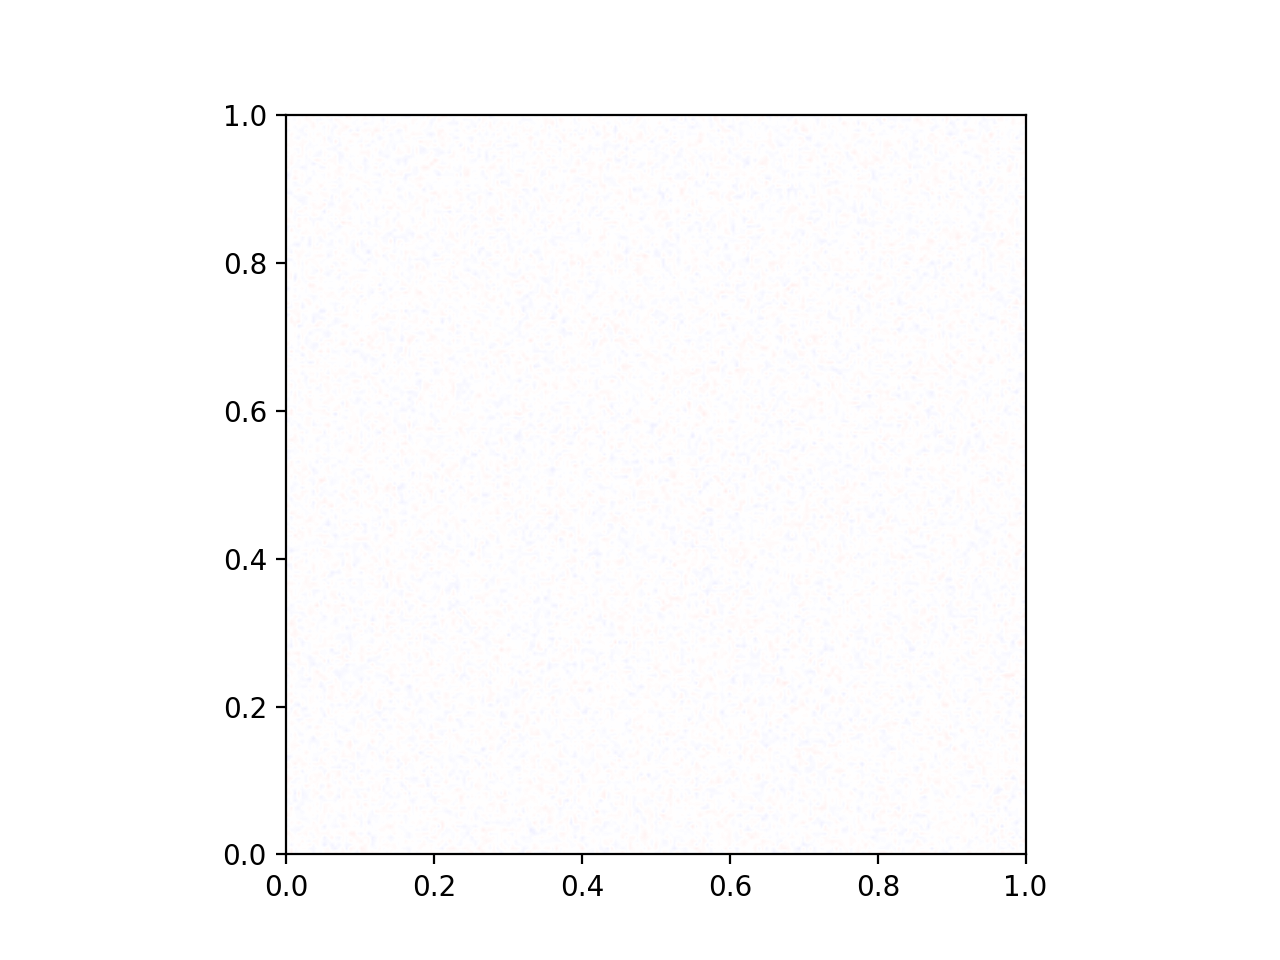
\includegraphics[width = 3in]{gif/test-0.png}
		\animategraphics[width = 3in, every = 1, loop]{6}{gif/test-}{0}{2}
	\end{figure}
\end{frame}

\section{Models}

\begin{frame}{Modeling Approaches}
	
	Continuum Model: Differential Equations
	\begin{itemize}
		\item Order parameter is a continuous quantity: \begin{equation}
			u\colon \Omega\times(0,\infty)\to[-1,1],\quad u\in\mathcal{C}^2
		\end{equation}
		\item Order parameter satisfies a single differential equation based on physical laws
		\item OUTPUT
	\end{itemize}

	Atomistic Model: Molecular Dynamics
	\begin{itemize}
		\item Collection of discrete classical particles
		\item Approximate interparticle forces are used to simulate Hamiltonian dynamics
		\item Generates trajectory of each particle
	\end{itemize}

\end{frame}

\begin{frame}{Model Type Comparison}

	Estimating the order parameter from molecular dynamics trajectory	
	
\end{frame}

\subsection{Differential Equations}

\begin{frame}{Heat Equation}
	
	The heat (or diffusion) equation with initial condition $u_0(x)$ and periodic boundary conditions
	\begin{equation} \label{eq_HE}
		\left\{
			\begin{split}
				&\frac{\partial u}{\partial t}=D\nabla^2u&x\in\Omega,t>0\\
				&u\big|_{x_i=0}=u\big|_{x_i=1}&1\le i\le d\\
				&u_{x_i}\big|_{x_i=0}=u_{x_i}\big|_{x_i=1}&1\le i\le d\\
				&u(x,0)=u_0(x)&x\in\Omega
			\end{split}	
		\right.
	\end{equation}
	
	
\end{frame}

\begin{frame}{Allen-Cahn Equation}
	
	The Allen-Cahn equation with initial condition $v_0(x)$ and periodic boundary conditions
	\begin{equation} \label{eq_AC}
		\left\{
			\begin{split}
				&\frac{\partial v}{\partial t}=\gamma\nabla^2v-\phi(v)&x\in\Omega,t>0\\
				&v\big|_{x_i=0}=v\big|_{x_i=1}&1\le i\le d\\
				&v_{x_i}\big|_{x_i=0}=v_{x_i}\big|_{x_i=1}&1\le i\le d\\
				&v(x,0)=v_0(x)&x\in\Omega
			\end{split}	
		\right.
	\end{equation}
	
\end{frame}

\begin{frame}{Cahn-Hilliard Equation}
	
	The Cahn-Hilliard equation with initial condition $c_0(x)$ and periodic boundary conditions


\end{frame}

\begin{frame}{Gradient Flow}

	Each equation we model can be viewed as the gradient flow of an energy functional $F$: 
	\begin{equation}
		\frac{\partial u}{\partial t}=-\frac{\partial F}{\partial u}	
	\end{equation}
	where $F\colon L^2(\Omega)\to\mathbb{R}$ for (\ref{eq_HE}) and (\ref{eq_AC}). For (\ref{eq_CH}), $F\colon H^{-1}(\Omega)\to\mathbb{R}$. The energy functionals are 
	\begin{equation}
		F(u)=\int_\Omega\frac{1}{2}|\nabla u|^2~\ud x
	\end{equation}
	for diffusion and 
	\begin{equation} \label{eq_func}
		F(v)=M\int_\Omega \psi(v)+\frac{\gamma}{2}|\nabla v|^2~\ud x
	\end{equation}
	for phase separation.
	
\end{frame}

\begin{frame}
	The function $\psi$ (\ref{eq_func}) is a double-well free energy function:
	\begin{equation}
		psi(v)=\frac{1}{4}(v^2-1)^2
	\end{equation}

	\begin{figure}
		\begin{center}
			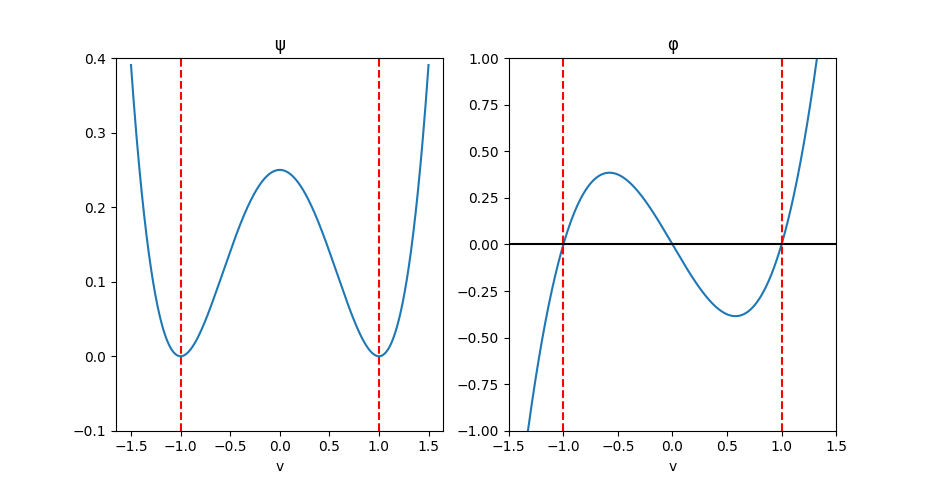
\includegraphics[width = 2in]{double_well_pot.png}
		\end{center}
	\end{figure}

	The minima of $\psi$ reflects the stability of phase separation. 
\end{frame}

\subsection{Molecular Dynamics}

\begin{frame}{Ideal Gas}


	
\end{frame}

\begin{frame}{Leonard-Jones Potential}


	\begin{itemize}
		\item Efficient and accurate model for pairiwise London Dispersion interparticle forces
		\item Parameters describe equilibrium distance and well depth
		\item Generally implemented with range cutoff
	\end{itemize}

	6-12 Leonard-Jones potential:
	\begin{equation}
		V(r)=4\epsilon\left[ \left( \frac{\sigma}{r} \right)^{12}-\left( \frac{\sigma}{r} \right)^6 \right]\quad r<r_c
	\end{equation}

	\begin{figure}
		\center
		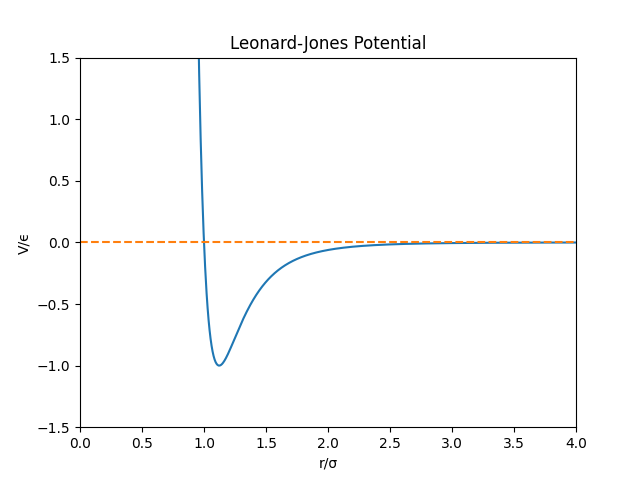
\includegraphics[width = 2in]{media/lj_pot.png}

	\end{figure}
	
\end{frame}

\begin{frame}{Leonard-Jones Fluid}
	
\end{frame}

\section{Numerical Methods}

\subsection{Finite Difference}

\begin{frame}{Difference Equations}
	
	Descretization of the domain:
	\begin{itemize}
		\item Divide
	\end{itemize}

\end{frame}

\begin{frame}{Stability}

	Stability conditions
	
\end{frame}

\begin{frame}{Convergence}
	
\end{frame}

\subsection{LAMMPS}



\end{document}